\scanpage{15}
\begingroup
\makeatletter
\tagsleft@true
\makeatother
\uline{\deleted{\unsure{I|V}}Version I}

% MARK01: observed full-scan bbox (191,141,195,145); local origin (191,141).
\unsure{\begin{tikzpicture}[baseline=0pt,x=.013cm,y=-.013cm]
\path[use as bounding box] (0,0) rectangle (74,8);
\fill (0,0) .. controls (2,-1) and (4,2) .. (4,4) .. controls (2,5) and (0,3) .. cycle;
\end{tikzpicture}}
Soient $X$ un espace topologique, $(\deleted{\unsure{\Sigma|S}}E_i)_{i\in I}$ un ens. de parties
% GUIDE01: full-scan origin (372,177), approximate curve within (371,214,475,261).
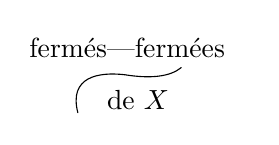
\begin{tikzpicture}[baseline=(opening.base),x=.013cm,y=-.013cm,line cap=round]
\path[use as bounding box] (-48,0) rectangle (170,87);
\node[anchor=base west,inner sep=0] at (-47,29) {\inserted{\unsure{fermés|fermées}}};
\node[anchor=base west,inner sep=0] (opening) at (29,80) {de $X$};
\draw (1,83) .. controls (-8,48) and (21,43) .. (47,46)
 .. controls (72,50) and (91,48) .. (102,39);
\end{tikzpicture}
(noté indiciellement), telles que l'on ait
% slanted
\reversemarginpar
\margin{$\nearrow$ On suppose de plus que pour \unsure{tte|toute|tt} comp. conn. $\unsure{\Sigma_i|\Sigma}$ de $X\setminus E_i$, on ait $\overline{\Sigma}_i\cap E_i\ne\varnothing$ i.e. $\overline{\Sigma}_i\ne\Sigma_i$ i.e. $\Sigma_i$ non fermé dans $X$ (ce qui est le cas si $X$ est connexe)}
\normalmarginpar
\[
 \forall i\in I,\quad \operatorname{Card}\pi_0(X\setminus\deleted{\Sigma}E_i)=2
 \tag*{(a)}
\]
% G02: separate upper horizontal stroke over the first Sigma in this NB.
% The overset rule preserves the stroke; its role remains undetermined.
\margin{\uline{NB} les comp. conn. $\overset{\unsure{\rule{.8em}{.35pt}}}{\Sigma}_i^+,\Sigma_i^{\unsure{+|-|\ast}}$ de $X\setminus\Sigma_i$ sont ouvertes dans $X$}
\[
 \begin{aligned}
 &\forall(i,j)\in I\times I,\ i\ne j,\quad \deleted{\Sigma}E_j\ \text{est contenu dans l'une}\\
 &\text{des deux composantes connexes de }X\setminus\deleted{\Sigma}E_i.
 \end{aligned}
 \tag*{(b)}
\]

NB Cette condition (b) est vérifiée automatiquement les $\deleted{\Sigma}E_i$ $(i\in I)$ sont connexes, dès lors que les $E_i$ sont supposés disjoints mutuellement

On se propose d'étudier le ``découpage'' de $X$ par la famille $(E_i)$.

% RULE01: full-scan origin (501,996); long wavy underline and separate short run under 2.
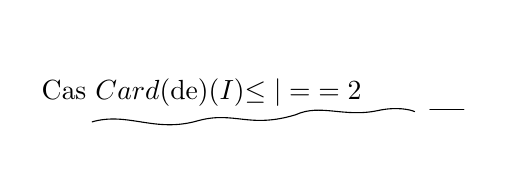
\begin{tikzpicture}[baseline=(case.base),x=.013cm,y=-.013cm,line cap=round]
\path[use as bounding box] (0,0) rectangle (443,117);
\node[anchor=base west,inner sep=0] (case) at (13,70)
 {Cas $\operatorname{Card}\deleted{\unsure{(\mathrm{de})}}(I)\deleted{\unsure{\leq|=}}=2$};
\draw (63,92) .. controls (98,82) and (124,103) .. (166,91)
 .. controls (202,81) and (216,99) .. (262,85)
 .. controls (286,74) and (309,88) .. (342,81)
 .. controls (360,77) and (374,80) .. (378,82);
\draw (393,80) -- (426,80);
\end{tikzpicture}

Soit $\Sigma_i^+$ la comp. conn. de $X\setminus E_i$ qui ne contient pas $E_j$ $(j\ne i)$, alors on a (si $I=\{1,2\}$)
% DRAW01: full-scan origin (19,1038), fixed local source-pixel rectangle.
% C's two left-brace paths and right-brace path are retained after checking,
% with local translation (5,33), i.e. full-scan origin (24,1071) for those paths.
\figure{\begin{tikzpicture}[x=.013cm,y=-.013cm,line cap=round,line join=round]
\path[use as bounding box] (0,0) rectangle (553,336);
% Oval: visible strong runs, pale runs and short gaps are distinct paths.
\draw (186,122) .. controls (210,76) and (262,35) .. (290,38)
 .. controls (342,35) and (380,88) .. (402,160);
\draw (403,168) .. controls (405,185) and (403,206) .. (401,216);
\draw[black!45] (401,217) .. controls (401,226) and (398,235) .. (394,243);
\draw (391,249) .. controls (387,257) and (382,263) .. (378,267);
\draw (374,273) .. controls (369,282) and (365,287) .. (361,291);
\draw (358,295) .. controls (334,319) and (294,320) .. (269,315)
 .. controls (219,309) and (178,276) .. (169,220)
 .. controls (166,206) and (168,197) .. (168,193);
\draw (168,193) .. controls (163,196) and (163,190) .. (166,181);
\draw (168,193) -- (173,185);
\draw[black!45] (168,179) .. controls (174,160) and (179,139) .. (186,122);
% Chords, separately checked at both rim contacts.
\draw[line width=.8pt] (186,122) .. controls (247,125) and (324,109) .. (392,119)
 (176,250) .. controls (242,253) and (328,246) .. (391,239);
\begin{scope}[shift={(5,33)}]
\draw (44,9) .. controls (46,57) and (63,106) .. (32,108)
 .. controls (52,132) and (38,151) .. (46,195) -- (55,228);
\draw (41,109) .. controls (72,143) and (35,144) .. (48,193)
 .. controls (47,224) and (57,241) .. (39,252) .. controls (55,242) and (43,259) .. (49,282);
\draw (428,86) .. controls (439,93) and (409,141) .. (434,149)
 .. controls (420,158) and (436,251) .. (417,254);
\end{scope}
% Cancelled label: one visible text copy, actual crossing paths, invisible deletion annotation.
\node[inner sep=0pt] at (167,48) {\rlap{$\unsure{\Sigma_1^+|\Sigma_2^+}$}\phantom{$\deleted{\unsure{\Sigma_1^+|\Sigma_2^+}}$}};
\draw (138,60) -- (198,27);
\draw (151,42) .. controls (161,20) and (181,12) .. (177,24) -- (149,52);
\node at (139,116) {$E_1$}; \node at (150,247) {$E_2$};
\node at (430,68) {$\Sigma_1^+$};
\node at (501,193) {$\Sigma_1^{\deleted{\unsure{+}}\unsure{-}}$};
\node at (23,135) {$\Sigma_2^-$}; \node at (131,308) {$\Sigma_2^+$};
% MARK01: detached short dot above the right overwritten superscript;
% full-scan observed bbox approximately (525,1189,531,1198), role/hand unresolved.
% Fixed inner origin: parent (507,153), full source (526,1191).
% Baseline 0 and base-west/zero-separation anchor map the inner origin exactly.
\node[anchor=base west,inner sep=0pt,outer sep=0pt] at (507,153) {\unsure{\begin{tikzpicture}[baseline=0pt,x=.013cm,y=-.013cm]
\path[use as bounding box] (0,0) rectangle (4,6);
\fill (1,0) .. controls (4,1) and (4,4) .. (2,6) .. controls (0,5) and (0,2) .. (1,0);
\end{tikzpicture}}};
\end{tikzpicture}}
\[
 \Sigma_1^+\cap\Sigma_2^+=\varnothing
 \tag*{(1)}
\]
ce qui \deleted{résulte de}
\[
 \begin{aligned}
 &\begin{tikzpicture}[baseline=(inc.base),x=.013cm,y=-.013cm,line cap=round]
 \path[use as bounding box] (0,0) rectangle (329,79);
 \node[anchor=base west,inner sep=0] (inc) at (2,59)
 {\rlap{$\Sigma_1^-\supset\Sigma_2^+$}\phantom{$\deleted{\Sigma_1^-\supset\Sigma_2^+}$}};
 % CANCEL02: original full-scan origin (704,1388).
 \draw (2,54) .. controls (149,38) and (243,44) .. (325,37);
 % MARK03: two detached points above the relation, observed (859,1404,863,1411).
 % Fixed inner origin: parent (155,16), full source (859,1404).
 \node[anchor=base west,inner sep=0pt,outer sep=0pt] at (155,16) {\unsure{\begin{tikzpicture}[baseline=0pt,x=.013cm,y=-.013cm]
 \path[use as bounding box] (0,0) rectangle (5,8);
 \fill (3,0) circle[radius=.8]; \fill (1,6) circle[radius=1];
 \end{tikzpicture}}};
 \end{tikzpicture}
 \qquad\text{\unsure{équivaut|èquivaut} à}\\
 &\deleted{\Sigma_2^-\supset\Sigma_1^+}\qquad \Sigma_1^+\subset\Sigma_2^-\cup E_2,\quad\text{et}
 \end{aligned}
\]
% CANCEL03: two distinct strokes, full-scan origin (202,1435).
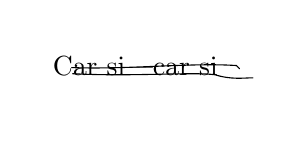
\begin{tikzpicture}[baseline=(carsi.base),x=.013cm,y=-.013cm,line cap=round]
\path[use as bounding box] (0,0) rectangle (231,83);
\node[anchor=base west,inner sep=0] (carsi) at (24,47)
 {\rlap{\unsure{Car si|car si}}\phantom{\deleted{\unsure{Car si|car si}}}};
\draw (43,39) .. controls (99,41) and (160,34) .. (204,37) -- (207,40);
\draw (44,45) .. controls (104,48) and (161,43) .. (183,46)
 .. controls (199,51) and (211,49) .. (220,49);
\end{tikzpicture}
\deleted{Si on avait} comme $\Sigma_1^+\cap E_2=\varnothing$, cela équivaut aussi à
\[
 \Sigma_1^+\subset\Sigma_2^-
 \tag*{(2)}
\]
% MARK04: independent right-side pair, full scan (1603,1778,1610,1786).
\margin{\unsure{\begin{tikzpicture}[x=.013cm,y=-.013cm]
\path[use as bounding box] (0,0) rectangle (9,10);
\fill (6,1) .. controls (8,0) and (9,2) .. (6,4) .. controls (4,4) and (4,2) .. cycle;
\fill (1,7) .. controls (3,6) and (5,7) .. (3,9) .. controls (1,9) and (0,8) .. cycle;
\end{tikzpicture}}}
\unsure{et} \unsure{symètriquement|symétriquement}, à
\[
 \Sigma_2^+\subset\Sigma_1^-
 \tag*{$(2')$}
\]

% Lower correction group: full-scan (x,y) = local (x+219,y+2009).
\figure{\begin{tikzpicture}[x=.009cm,y=-.009cm,line cap=round,line join=round]
\path[use as bounding box] (0,0) rectangle (1448,145);
\node[anchor=base west,inner sep=0] at (19,122) {Comme};
\node[anchor=base west,inner sep=0] at (207,43) {\rlap{\unsure{vois. ouvert}}\phantom{\deleted{\unsure{vois. ouvert}}}};
\draw (209,37) .. controls (270,33) and (334,38) .. (410,36);
\node[anchor=base west,inner sep=0] at (265,122) {$\Sigma_2^-\supset E_1,$};
% Selected C MARK02 body; fixed inner full origin (510,2061).
% Parent origin (219,2009), anchor (291,52); wrapper units match the parent.
\node[anchor=base west,inner sep=0pt,outer sep=0pt] at (291,52) {\unsure{\begin{tikzpicture}[baseline=0pt,x=.009cm,y=-.009cm,line cap=round]
\path[use as bounding box] (0,0) rectangle (19,16);
\draw[line width=.6pt] (1,15) .. controls (8,7) and (13,3) .. (18,2);
\end{tikzpicture}}};
\node[anchor=base west,inner sep=0] at (556,97) {\rlap{il contient les}\phantom{\deleted{il contient les}}};
\draw (557,91) .. controls (705,95) and (858,86) .. (997,82);
\node[anchor=base west,inner sep=0] at (557,49) {\inserted{i.e. $\Sigma_2^-$ est un \uline{vois}. ouvert de $E_1$,}};
\node[anchor=base west,inner sep=0] at (1048,93) {on \unsure{a}};
\end{tikzpicture}}
% slanted; local note coordinates are full-scan coordinates minus (17,1962).
% A GUIDE02 short arrow and C GUIDE02 long curve are separate locally qualified components.
\reversemarginpar
\margin{\figure{\begin{tikzpicture}[x=.009cm,y=-.009cm,line cap=round]
\path[use as bounding box] (0,0) rectangle (445,383);
\node[rotate=40,inner sep=0] at (114,154) {$\overline{\Sigma_1^+}\cap E_1\ne\varnothing$};
\node[rotate=40,inner sep=0] at (264,56) {i.e.};
\node[rotate=40,inner sep=0] at (95,260) {$\overline{\Sigma_1^+}\ne\Sigma_1^+$};
\node[rotate=40,inner sep=0] at (331,85) {\unsure{à sign.ler|à signaler}};
\node[rotate=40,inner sep=0] at (94,326) {avant};
% Approximate paths: GUIDE02 observed near (233,2071)-(274,2131).
% A GUIDE02 locally qualified; its attachment/role/hand/origin remain undetermined.
% Wrapper anchor and opposite inner shift preserve the two original path bodies.
\node[anchor=base west,inner sep=0pt,outer sep=0pt] at (211,103) {\unsure{\begin{tikzpicture}[baseline=0pt,x=.009cm,y=-.009cm,line cap=round]
\path[use as bounding box] (0,0) rectangle (50,70);
\begin{scope}[shift={(-211,-103)}]
\draw (257,110) .. controls (224,103) and (211,125) .. (217,144)
 .. controls (222,149) and (233,150) .. (237,168);
\draw (237,168) -- (227,162) (237,168) -- (238,156);
\end{scope}
\end{tikzpicture}}};
% Selected C GUIDE02 replaces A GUIDE03; one longer curve is supplied.
% Fixed inner origin in note (163,196), full source (180,2158).
\node[anchor=base west,inner sep=0pt,outer sep=0pt] at (163,196) {\unsure{\begin{tikzpicture}[baseline=0pt,x=.009cm,y=-.009cm,line cap=round]
\path[use as bounding box] (0,0) rectangle (125,67);
\draw[black!65] (7,59) .. controls (0,34) and (22,28) .. (60,21)
 .. controls (87,18) and (105,13) .. (118,7);
\end{tikzpicture}}};
\end{tikzpicture}}}
\normalmarginpar
\[
 \Sigma_2^-\cap\Sigma_1^+\ne\varnothing
\]
Car
% RULE02: hooked short underline, observed full bbox (896,2226,1038,2245).
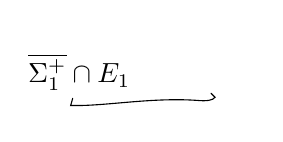
\begin{tikzpicture}[baseline=(carformula.base),x=.013cm,y=-.013cm,line cap=round]
\path[use as bounding box] (0,-54) rectangle (222,30);
\node[anchor=base west,inner sep=0] (carformula) at (0,0) {$\overline{\Sigma_1^+}\cap E_1$};
\draw (44,15) -- (42,22) .. controls (75,23) and (119,14) .. (165,17)
 .. controls (175,18) and (181,17) .. (183,14) -- (179,10);
\end{tikzpicture}
$\ne\varnothing$
% Final local insertion: coordinates are full scan minus (1278,2080).
\figure{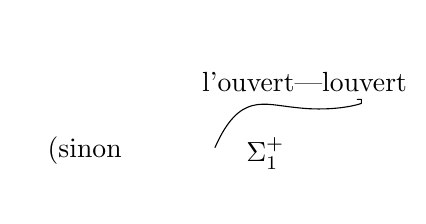
\begin{tikzpicture}[x=.013cm,y=-.013cm,line cap=round,line join=round]
\path[use as bounding box] (0,0) rectangle (362,164);
\node[anchor=base west,inner sep=0] at (19,127) {(sinon};
\node[anchor=base west,inner sep=0] at (170,62) {\inserted{\unsure{l'ouvert|louvert}}};
\node[anchor=base west,inner sep=0] at (213,131) {$\Sigma_1^+$};
% GUIDE02: bent attachment guide from before Sigma to the right of the inserted word.
\draw (183,117) .. controls (207,63) and (230,75) .. (262,78)
 .. controls (285,81) and (311,79) .. (326,74) -- (326,70) -- (322,70);
\end{tikzpicture}}
serait \inserted{un} fermé dans $X$, \unsure{donc|puis}
% CANCEL03: full-scan origin (920,2238), one text copy and visible overstrikes.
\begin{tikzpicture}[x=.013cm,y=-.013cm,baseline=(del.base),line cap=round,line join=round]
\path[use as bounding box] (0,0) rectangle (177,67);
\node[anchor=base west,inner sep=0pt] (del) at (16,49) {\rlap{$\unsure{\Sigma_1^+\text{ serait}|\Sigma_1^+\ne\varnothing}$}\phantom{$\deleted{\unsure{\Sigma_1^+\text{ serait}|\Sigma_1^+\ne\varnothing}}$}};
\draw (14,31) -- (53,9);
\draw (8,25) -- (18,5) -- (24,29) -- (39,23);
\draw (24,32) .. controls (60,23) and (105,29) .. (164,39);
% Only B G07's second short upright is added; C's angular path remains once.
% Fixed inner origin in C's group (12,1), full source (932,2239).
\node[anchor=base west,inner sep=0pt,outer sep=0pt] at (12,1) {\unsure{\begin{tikzpicture}[baseline=0pt,x=.013cm,y=-.013cm,line cap=round]
\path[use as bounding box] (0,0) rectangle (37,24);
\draw (24,6) -- (26,16);
\end{tikzpicture}}};
\end{tikzpicture} $X$ serait disconnexe),
\endgroup
% archive sheet number: 14
